\documentclass{article}
\usepackage{graphicx}
\usepackage{tikz}
\begin{document}

\begin{center}

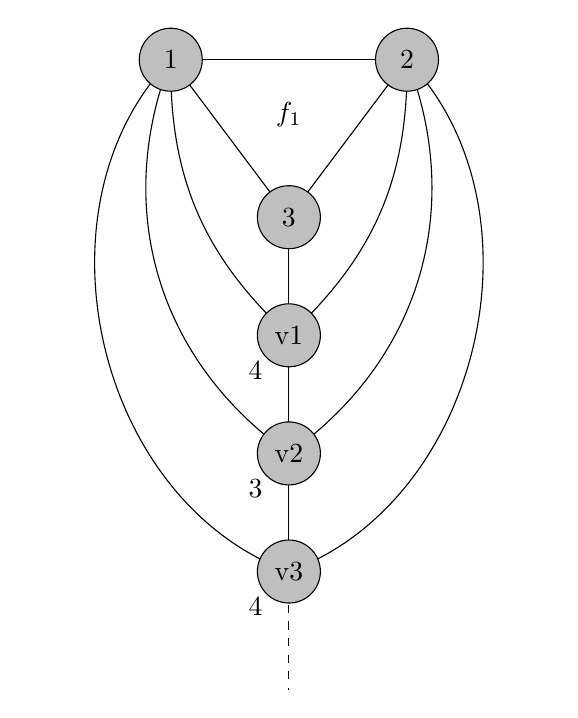
\begin{tikzpicture}
  \draw (2,14) -- (5,14)
  node[midway, yshift=-0.7cm]{$f_1$};
  \draw (2,14) -- (3.5,12);
  \draw (5,14) -- (3.5,12);
  \draw (2,14) to[bend right=24] (3.5,10.5);
  \draw (2,14) to[bend right=38] (3.5,9);
  \draw (2,14) to[bend right=57] (3.5,7.5);
  \draw (5,14) to[bend left=24] (3.5,10.5);
  \draw (5,14) to[bend left=38] (3.5,9);
  \draw (5,14) to[bend left=57] (3.5,7.5);
  \draw (3.5,12) -- (3.5,10.5);
  \draw (3.5,10.5) -- (3.5,9);
  \draw (3.5,9) -- (3.5,7.5);
  \draw[dashed] (3.5,7.5) -- (3.5,6);
  \filldraw[fill=lightgray] (2,14) circle (0.4) node{1};
  \filldraw[fill=lightgray] (5,14) circle (0.4) node{2};
  \filldraw[fill=lightgray] (3.5,12) circle (0.4) node{3};
  \filldraw[fill=lightgray] (3.5,10.5) circle (0.4) 
    node{v1}
    node[below left=6pt]{4};
  \filldraw[fill=lightgray] (3.5,9) circle (0.4) 
    node{v2}
    node[below left=6pt]{3};
  \filldraw[fill=lightgray] (3.5,7.5) circle (0.4)
    node{v3}
    node[below left=6pt]{4};;
\end{tikzpicture}

\end{center}
\end{document}
